%%
%% This is file `sample-sigplan.tex',
%% generated with the docstrip utility.
%%
%% The original source files were:
%%
%% samples.dtx  (with options: `sigplan')
%% 
%% IMPORTANT NOTICE:
%% 
%% For the copyright see the source file.
%% 
%% Any modified versions of this file must be renamed
%% with new filenames distinct from sample-sigplan.tex.
%% 
%% For distribution of the original source see the terms
%% for copying and modification in the file samples.dtx.
%% 
%% This generated file may be distributed as long as the
%% original source files, as listed above, are part of the
%% same distribution. (The sources need not necessarily be
%% in the same archive or directory.)
%%
%%
%% Commands for TeXCount
%TC:macro \cite [option:text,text]
%TC:macro \citep [option:text,text]
%TC:macro \citet [option:text,text]
%TC:envir table 0 1
%TC:envir table* 0 1
%TC:envir tabular [ignore] word
%TC:envir displaymath 0 word
%TC:envir math 0 word
%TC:envir comment 0 0
%%
%%
%% The first command in your LaTeX source must be the \documentclass command.
\documentclass[sigplan,screen]{acmart}

%%
%% \BibTeX command to typeset BibTeX logo in the docs
\AtBeginDocument{%
  \providecommand\BibTeX{{%
    Bib\TeX}}}

%% Rights management information.  This information is sent to you
%% when you complete the rights form.  These commands have SAMPLE
%% values in them; it is your responsibility as an author to replace
%% the commands and values with those provided to you when you
%% complete the rights form.
\setcopyright{rightsretained}
\copyrightyear{2022}
%\acmYear{2018}
%\acmDOI{XXXXXXX.XXXXXXX}

%% These commands are for a PROCEEDINGS abstract or paper.
%acmConference[Machine Learning for Behavioural Data (CS-421)]{}{12th of June,
 % 2022}{Lausanne, CH}
%\acmPrice{15.00}
%\acmISBN{978-1-4503-XXXX-X/18/06}


%%
%% Submission ID.
%% Use this when submitting an article to a sponsored event. You'll
%% receive a unique submission ID from the organizers
%% of the event, and this ID should be used as the parameter to this command.
%%\acmSubmissionID{123-A56-BU3}

%%
%% For managing citations, it is recommended to use bibliography
%% files in BibTeX format.
%%
%% You can then either use BibTeX with the ACM-Reference-Format style,
%% or BibLaTeX with the acmnumeric or acmauthoryear sytles, that include
%% support for advanced citation of software artefact from the
%% biblatex-software package, also separately available on CTAN.
%%
%% Look at the sample-*-biblatex.tex files for templates showcasing
%% the biblatex styles.
%%

%%
%% The majority of ACM publications use numbered citations and
%% references.  The command \citestyle{authoryear} switches to the
%% "author year" style.
%%
%% If you are preparing content for an event
%% sponsored by ACM SIGGRAPH, you must use the "author year" style of
%% citations and references.
%% Uncommenting
%% the next command will enable that style.
%%\citestyle{acmauthoryear}

\usepackage{csquotes}

%%
%% end of the preamble, start of the body of the document source.
\begin{document}

%%
%% The "title" command has an optional parameter,
%% allowing the author to define a "short title" to be used in page headers.
\title[Do As I Do]{Do As I Do -- more scientific follow up}

%%
%% The "author" command and its associated commands are used to define
%% the authors and their affiliations.
%% Of note is the shared affiliation of the first two authors, and the
%% "authornote" and "authornotemark" commands
%% used to denote shared contribution to the research.
\author{Kai Cooper}
\authornote{All authors contributed equally to this research.}
\affiliation{%
  \institution{EPFL, Mathematics (exchange from Imperial College London)}
  \city{Lausanne}
  \state{Vaud}
  \country{Switzerland}
}
\email{kai.cooper@epfl.ch}

\author{Nicolas d'Argenlieu}
\authornotemark[1]
\affiliation{%
  \institution{EPFL, Data Science (Master)}
  \city{Lausanne}
  \state{Vaud}
  \country{Switzerland}}
\email{nicolas.thierrydargenlieu@epfl.ch}

\author{Mar\'ia Isabel Ruiz Mart\'inez}
\authornotemark[1]
\affiliation{%
  \institution{EPFL, Computer Science (exchange from Universidad de Grenada)}
  \city{Lausanne}
  \state{Vaud}
  \country{Switzerland}
}
\email{maria.ruizmartinez@epfl.ch}


%%
%% By default, the full list of authors will be used in the page
%% headers. Often, this list is too long, and will overlap
%% other information printed in the page headers. This command allows
%% the author to define a more concise list
%% of authors' names for this purpose.
\renewcommand{\shortauthors}{Cooper et al.}

%%
%% The abstract is a short summary of the work to be presented in the
%% article.
\begin{abstract}
In this report, we present the results of a learning analytics study. The data analysed are produced by chronologically recorded clickstreams of Swiss secondary school student usage of the online maths and German learning platform Lernnavi. We quantify student behavioural patterns, in particular their regularity, and use these features to predict student attainment on the platform through a supervised learning pipeline. Our results reinforce that regular and persistent usage of the platform leads to better performance, however our models also serve to highlight some of the pitfalls of aiming to study human behaviour through opaque clickstreams. 
\end{abstract}

%%
%% Keywords. The author(s) should pick words that accurately describe
%% the work being presented. Separate the keywords with commas.
\keywords{datasets, regularity, decision trees, time series classification, prediction, clustering, lernnavi, moocs, education, student attainment}
%% A "teaser" image appears between the author and affiliation
%% information and the body of the document, and typically spans the
%% page.
\begin{teaserfigure}
  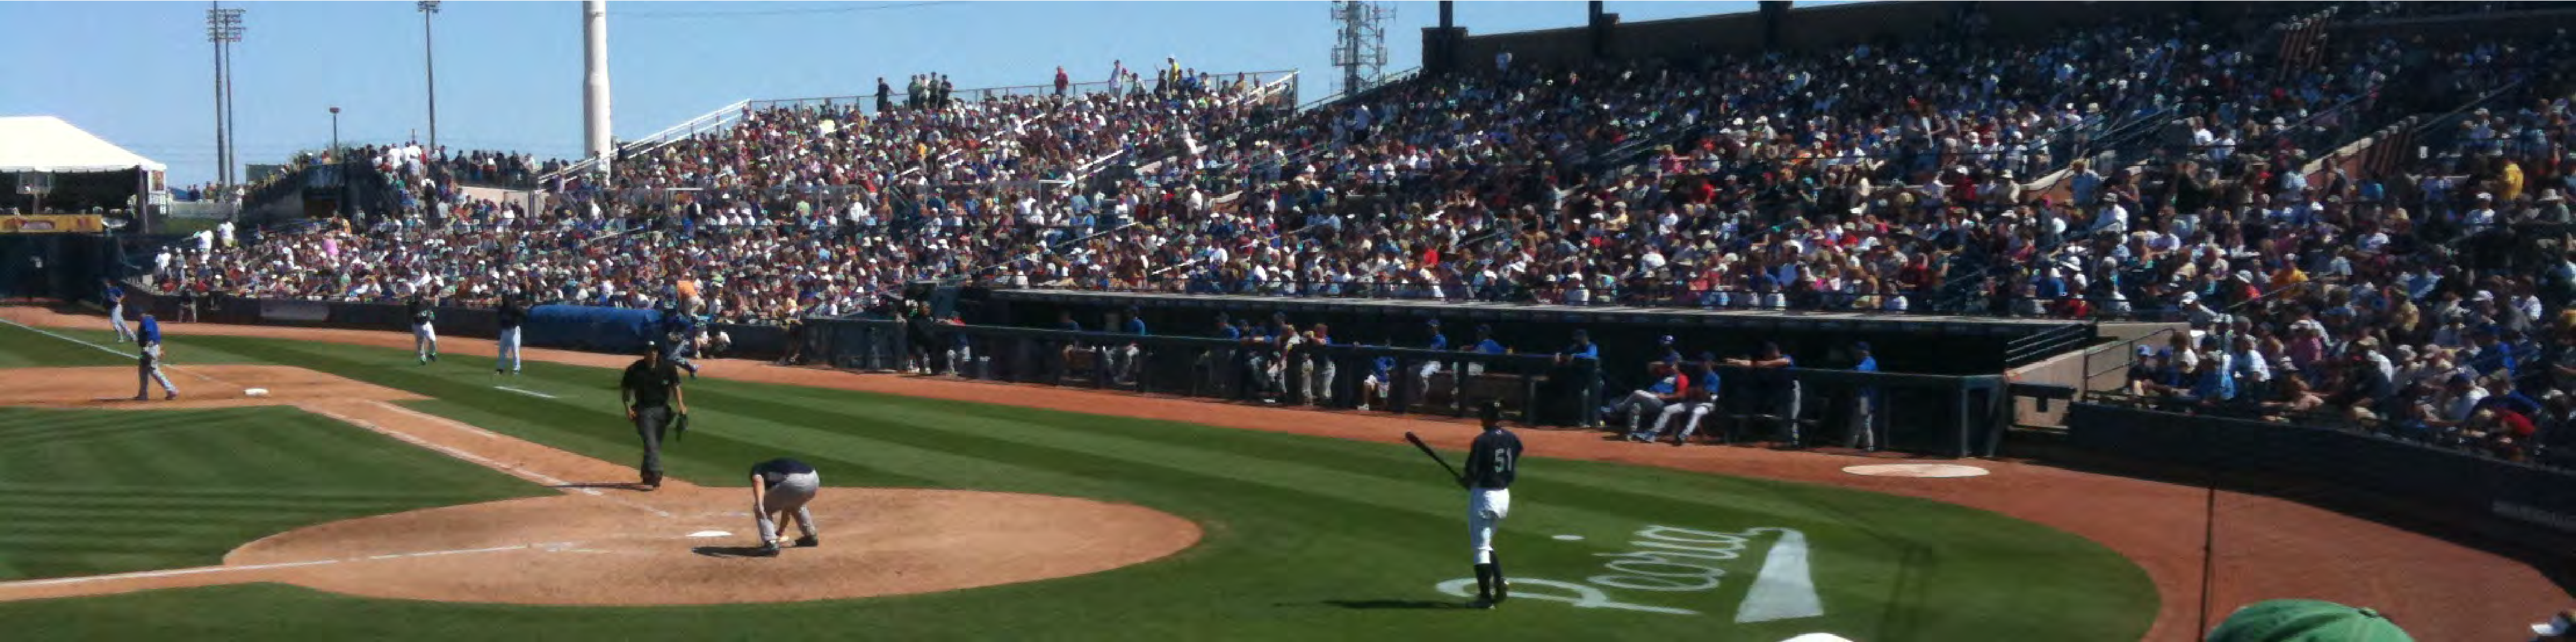
\includegraphics[width=\textwidth]{reports/figures/sampleteaser.pdf}
  \caption{Seattle Mariners at Spring Training, 2010.}
  \Description{Enjoying the baseball game from the third-base
  seats. Ichiro Suzuki preparing to bat.}
  \label{fig:teaser}
\end{teaserfigure}

%%
%% This command processes the author and affiliation and title
%% information and builds the first part of the formatted document.
\maketitle

\section{Introduction}
Improved digital technologies have made online learning formats such as MOOCs and dedicated learning platforms such as Moodle more accessible. Lernnavi is one of these online education platforms, whose primary use is as an accompanying teaching and learning tool in secondary education. They offer maths and German lessons and exercises. Students track their progress through a mastery score updated by so-called \textbf{level checks}, unique to each topic taught on the platform. 

\subsection{Research Question}

Innately, we are all aware of the fact that self-improvement demands commitment. This notion is omnipresent in education and is a persistent device used by educators to encourage learning. Consequently, we anticipate that students who choose (or are perhaps forced) to exhibit regular, recurrent patterns of learning behaviours will experience greater learning gains in the long-run. In this project, we wish to discover if this phenomenon is present within the Lernnavi environment, while going to a step further and identify which specific behaviours \textit{may} lead to higher attainment for a given student. In light of this, we state our research question:

\begin{displayquote}
\textit{Is it possible to identify one or more studying behaviors leading to a significant improvement in level check results?}
\end{displayquote}



\section{Data Description and Exploratory Analysis}

{\color{red}
\begin{itemize}
    \item Data description in its \textbf{most raw form}: what the different tables are and their contents (overview); shape of most important datasets.
    \item Exploratory analysis based on the above.
    \item \textbf{Note: for the above, much has already been done.} 
\end{itemize}
}

\begin{figure}
    \centering
    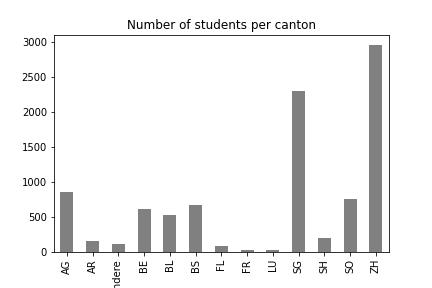
\includegraphics[width=\linewidth]{reports/figures/num_per_canton.jpg}
    \caption{Caption}
    \label{fig:my_label}
\end{figure}

\begin{figure*}[!ht]
    \centering
    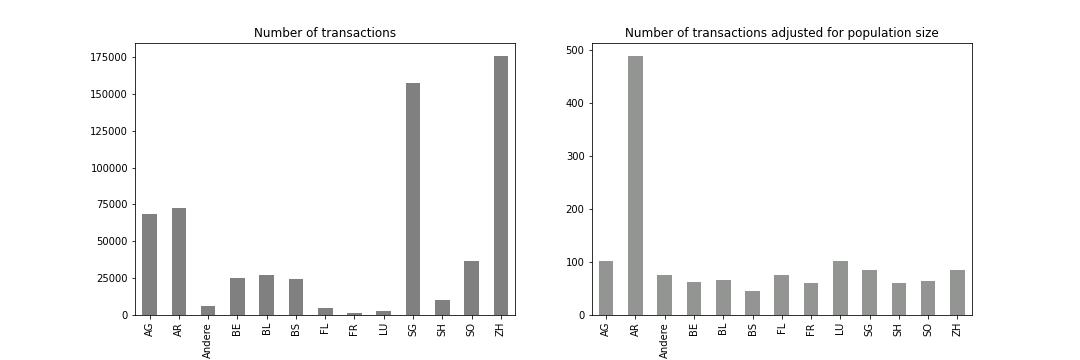
\includegraphics[width=\linewidth]{reports/figures/cantonal_representation.jpg}
    \caption{Caption}
    \label{fig:cantonal_representation}
\end{figure*}


\section{The Proposed Approach}

{\color{red}
\begin{itemize}
    \item Data cleaning approaches: what is removed and rationale; changes in shape of dataset.
\end{itemize}
}
\subsection{A1}
{\color{red}Description of methodology.}
Clustering is performed based on a set of time agnostic features for each user. These features include: counts of each significant action (an action with a transaction token); length of time on the platform, and a set of so-called \textbf{regularity} features. The latter is a set of metrics which measure to what extent user patterns repeat of chosen time periods, for example over hours of the day, days of the week, or weeks of the month. For instance, one feature, \texttt{PDH} -- an abbreviation of \textit{peak on day hour} -- measures if a users activity is concentrated around certain times of the day, based on the entropy of the histogram of the user's daily activity. We refer the reader to \cite{quantifyreg} to find a detailed description of all of the features.
\subsection{A2}
{\color{red}Description of methodology.}     
\begin{table*}[!ht]
  \caption{Time agnostic, aggregated features used in methodology A2 for a given user $i$ for all data recorded on the platform before level check $j$.}
  \label{tab:A2features}
  \begin{tabular}{cl}
    \toprule
    \textbf{Feature}&\textbf{Description}\\
    \midrule
    $\texttt{num\_weeks\_on}$ & number of weeks recorded having used the platform\\
    $\texttt{num\_actions\_per\_week}$ & average number of actions with a transaction token per week\\
    $\texttt{FDH}$ & measures the extent to which the hourly pattern of user’s activities is repeating over days \\
    $\texttt{FWH}$ & measures if the hourly pattern of activities is repeating over weeks\\
    $\texttt{FWD}$ & captures if the daily pattern of activities is repeating over weeks\\
    $\texttt{eng\_score}$ & binary indicator of `high' user engagement\\
    \bottomrule
    \end{tabular}
\end{table*}

\begin{figure}
    \centering
    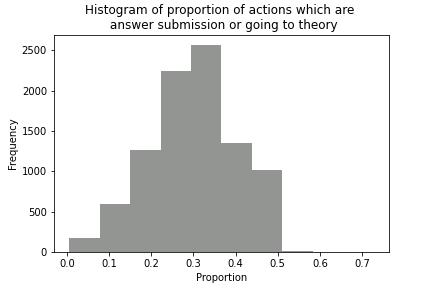
\includegraphics[width=\linewidth]{reports/figures/eng_score_hist.jpg}
    \caption{Caption}
    \label{fig:eng_score}
\end{figure}


\begin{figure}
    \centering
    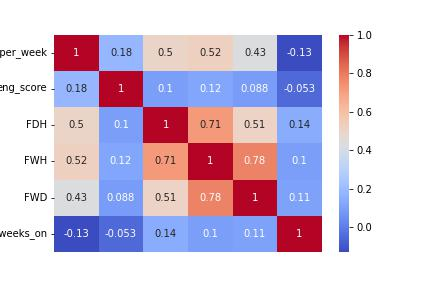
\includegraphics[width=\linewidth]{reports/figures/feature_corr.jpg}
    \caption{Correlation heatmap between all the features. Note we have relabelled $\texttt{num\_actions\_per\_week}$ to \#actions and $\texttt{num\_weeks\_on}$ to \#weeks for display purposes.}
    \label{fig:feature_corr}
\end{figure}


{\color{red}Clustering...}

A decision tree classifier based on behavioural features was chosen due to the very interpretable nature of such a model. Indeed, it allows for the categorisation of students based on quantitative metrics on usage of the platform, while also ranking the importance of the behavioural features, which help us in answering our research question. 

Let $N$ be the number of users and $L_i$ be the number of level checks user $i$ has completed. For every $i \in N$ and $j \in L_i$, the data fed into the decision tree classifier is a vector $x_i^j = (x_{i1}^j, x_{i2}^j, \ldots, x_{i6}^j)$ where $x_{i1}$ is a positive integer, $x_{ik}$ for $k=2,3,4$ is a positive real number and $x_{i6} \in \{0,1\}$. The features $x_{ik}$ for $k=1,\ldots, 6$ are listed in Table 
\ref{tab:A2features}. Mention/describe: {\color{red}Regularity features...}. An `engagement score`, inspired by \cite{student_engagement}, recors whether a student demonstrated that they performed activities directly related to learning (submitting answers to questions and going to theory sections of the app) more than other students. To quantify this, if for a given user, the two aforementioned actions comprised more than $25\%$ of all actions recorded in $\texttt{num\_actions\_per\_week}$, then they were given an engagement score of $1$ and $0$ otherwise. We remark that each of these features aim to quantify some form of consistent behavioural pattern on the platform, ranging from simply being present on the platform, to using it in a repeated manner over a long period of time. 

\section{Results}

\subsection{Experimental Evaluation}

The ``\verb|acmart|'' document class requires the use of the
``Libertine'' typeface family. Your \TeX\ installation should include
this set of packages. Please do not substitute other typefaces. The
``\verb|lmodern|'' and ``\verb|ltimes|'' packages should not be used,
as they will override the built-in typeface families.

\section{Discussion}

Our results demonstrate that differing patterns of student behaviours certainly influence their performance on the platform. Even as we could not identify a specific optimal behavior, both experiments clearly demonstrated its potential by giving good prediction accuracy. We believe that in future work, this platform could be used to carry out directed causal experiments where students demonstrate explicit patterns and use the technology to study what brings about student success.


The title of your work should use capital letters appropriately -
\url{https://capitalizemytitle.com/} has useful rules for
capitalization. Use the {\verb|title|} command to define the title of
your work. If your work has a subtitle, define it with the
{\verb|subtitle|} command.  Do not insert line breaks in your title.

If your title is lengthy, you must define a short version to be used
in the page headers, to prevent overlapping text. The \verb|title|
command has a ``short title'' parameter:
\begin{verbatim}
  \title[short title]{full title}
\end{verbatim}

\section{Conclusions and Future Works}

Each author must be defined separately for accurate metadata
identification.  As an exception, multiple authors may share one
affiliation. Authors' names should not be abbreviated; use full first
names wherever possible. Include authors' e-mail addresses whenever
possible.

Grouping authors' names or e-mail addresses, or providing an ``e-mail
alias,'' as shown below, is not acceptable:
\begin{verbatim}
  \author{Brooke Aster, David Mehldau}
  \email{dave,judy,steve@university.edu}
  \email{firstname.lastname@phillips.org}
\end{verbatim}

The \verb|authornote| and \verb|authornotemark| commands allow a note
to apply to multiple authors --- for example, if the first two authors
of an article contributed equally to the work.

If your author list is lengthy, you must define a shortened version of
the list of authors to be used in the page headers, to prevent
overlapping text. The following command should be placed just after
the last \verb|\author{}| definition:
\begin{verbatim}
  \renewcommand{\shortauthors}{McCartney, et al.}
\end{verbatim}
Omitting this command will force the use of a concatenated list of all
of the authors' names, which may result in overlapping text in the
page headers.

The article template's documentation, available at
\url{https://www.acm.org/publications/proceedings-template}, has a
complete explanation of these commands and tips for their effective
use.

Note that authors' addresses are mandatory for journal articles.


the margin:
\begin{description}
\item[\texttt{sidebar}:]  Place formatted text in the margin.
\item[\texttt{marginfigure}:] Place a figure in the margin.
\item[\texttt{margintable}:] Place a table in the margin.
\end{description}

%%
%% The acknowledgments section is defined using the "acks" environment
%% (and NOT an unnumbered section). This ensures the proper
%% identification of the section in the article metadata, and the
%% consistent spelling of the heading.
\begin{acks}
To Paola, for the sustained interest and really fruitful and engaging topical discussions.
\end{acks}

%%
%% The next two lines define the bibliography style to be used, and
%% the bibliography file.
\bibliographystyle{ACM-Reference-Format}
\bibliography{reports/refs.bib}


%%
%% If your work has an appendix, this is the place to put it.
\appendix

\section{Online Resources}

\begin{itemize}
    \item Python resources discussion here?
\end{itemize}




\end{document}
\endinput
%%
%% End of file `sample-sigplan.tex'.
